\subsection*{Report 1}

	A step and impulse response was convoluted with a transfer function of a high pass and low pass filter, with coefficient "a" being 0.95 and -0.95 for each respective filter. The MATLAB script used can be found on page \pageref{matlab_1.1}. The original input signals can be seen below in figure \ref{figure:1_1_1}. N was chosen as 100 samples, as the increased resolution gives a better indication on the nature of the responses.
	
	\begin{figure}[H] 
		\centering
		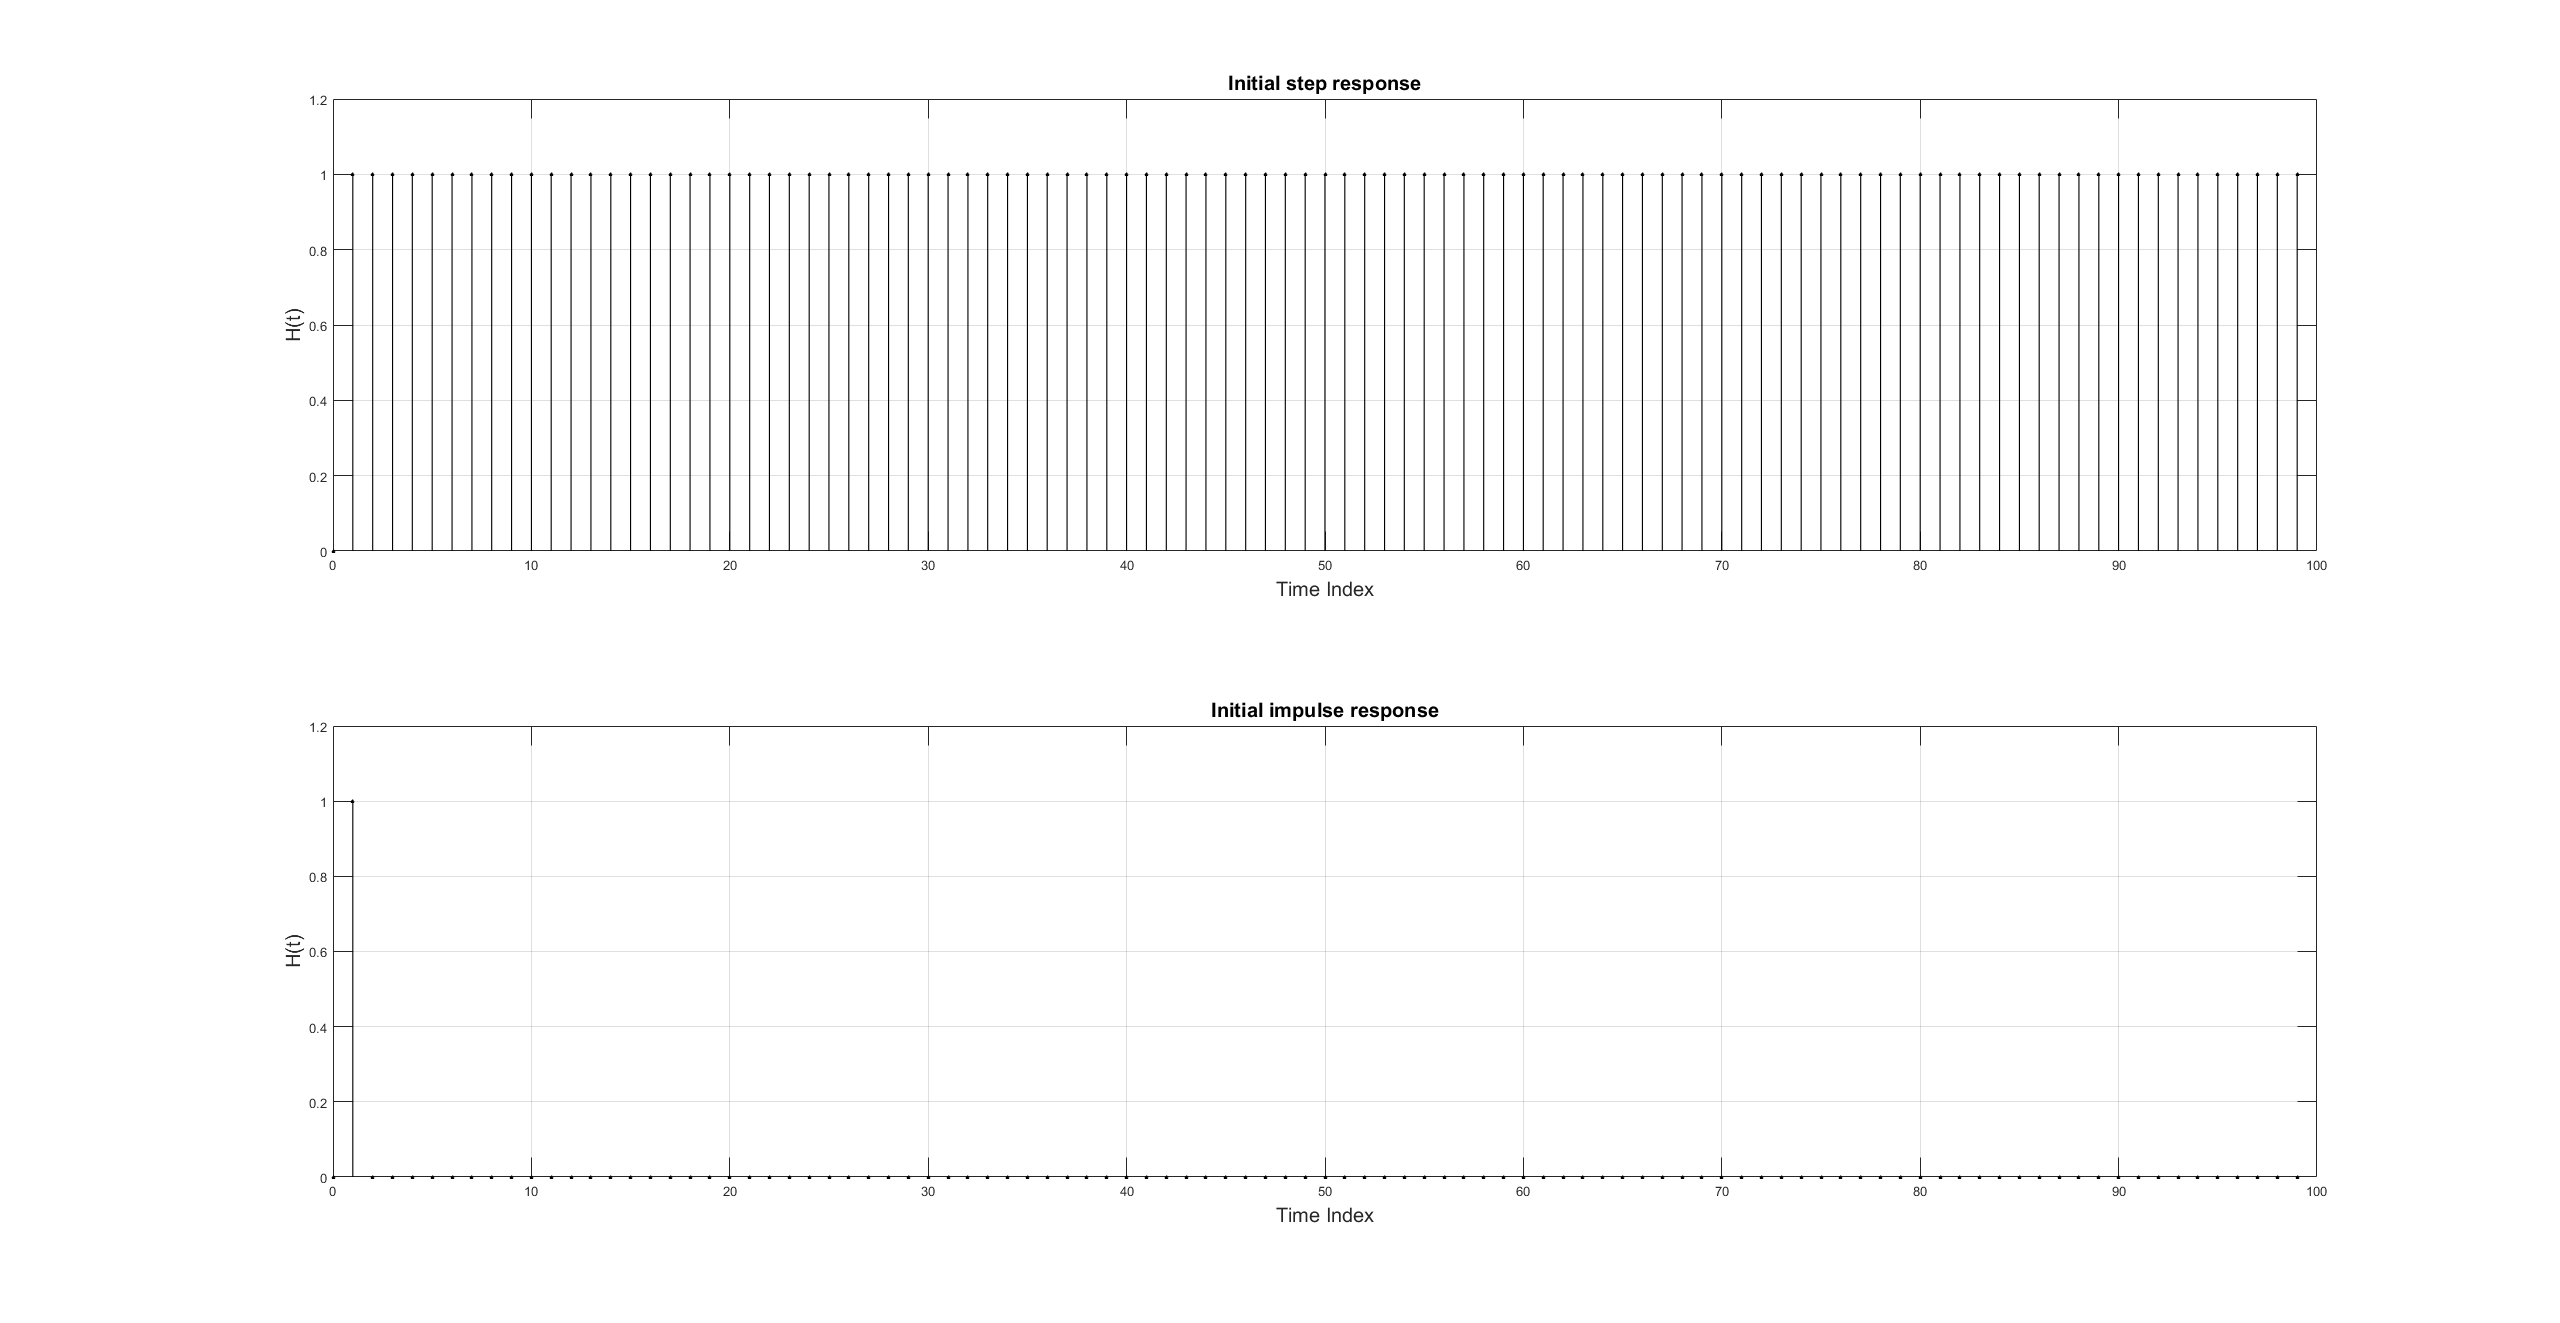
\includegraphics[width=\textwidth]{1.1.1.png}
		\caption{Input Impulse and Step Response}
		\label{figure:1_1_1}
	\end{figure}
	
	For the low pass signal response as seen in figure \ref{figure:1_1_2}, the step response (which contains very high frequency components) in filtered, which only leaves the low frequecy components, meaning the filter takes a while to equalize (reach the input value), which is typical of a low pass filter. Similarly, the impulse response shows the effective settling time of the filter after an impulse, dependant on the filter coefficient.
	
	\begin{figure}[H] 
		\centering
		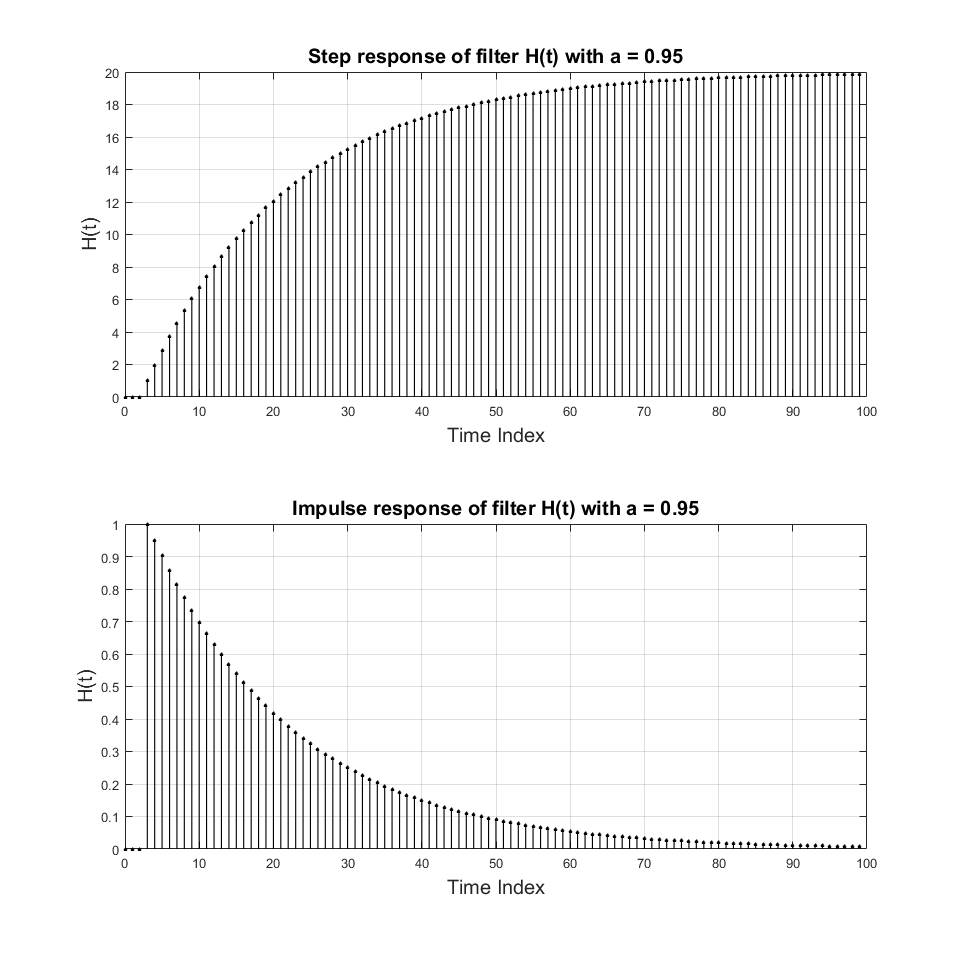
\includegraphics[width=\textwidth]{1.1.2.png}
		\caption{Low Pass Filter Response with a=0.95}
		\label{figure:1_1_2}
	\end{figure}

	For the high pass signal response as seen in figure \ref{figure:1_1_3}, the difference in amplitude for the step response is magnified greatly, as the high frequency content of the filter allows for the quick rise time. However, as these frequencies are not dampened by the filter, they dent to oscillate, which can also be seen in the figure. The impulse signal results as shows an oscillatory behaviour, as the high frequency components of the impulse are greatly magnified, but not dampened.
	
	\begin{figure}[H] 
		\centering
		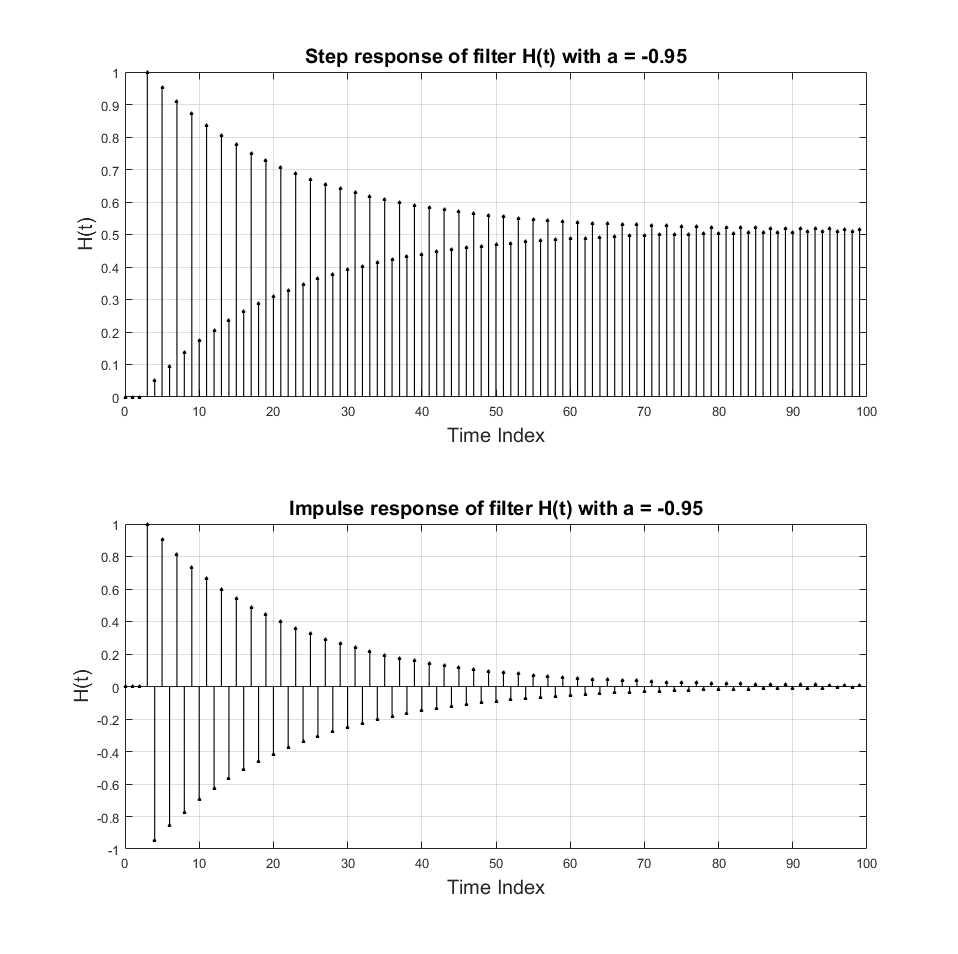
\includegraphics[width=\textwidth]{1.1.3.png}
		\caption{High Pass Filter Response with a=-0.95}
		\label{figure:1_1_3}
	\end{figure}